
\begin{frame}{malware}
    \begin{itemize}
    \item ``evil software''
    \item<2-> display a funny message
    \item<2-> send passwords/credit card numbers to criminals
    \item<2-> take pictures to send to criminals
    \item<2-> delete data
    \item<2-> hold data hostage
    \item<2-> insert/replace ads in webpages
    \item<2-> \ldots
    \end{itemize}
\end{frame}


\begin{frame}{viruses}
    \begin{itemize}
    \item malware that \myemph{inserts itself into another program}
    \item ``infects'' other programs when run
    \begin{itemize}
    \item usually modifies executables directly
    \end{itemize}
    \end{itemize}
\end{frame}

\begin{frame}{macro viruses}
    \begin{itemize}
    \item Word, Excel, other office software support \myemph{macros}
        \begin{itemize}
        \item scripts embedded in Word/Excel/etc. documents
        \end{itemize}
    \item viruses written in a \myemph{scripting language} 
        \begin{itemize}
        \item Visual Basic for Applications
        \end{itemize}
    \item spread to office documents, not executables
        \begin{itemize}
        \item easily spread in corporate environments
        \end{itemize}
    \item vendor reaction: macros disabled by default now
    \end{itemize}
\end{frame}

{ % all template changes are local to this group.
    \setbeamertemplate{navigation symbols}{}
    \begin{frame}[plain]
        \begin{tikzpicture}[remember picture,overlay]
            \node[at=(current page.center)] {
                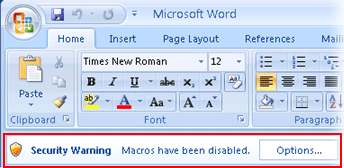
\includegraphics[width=\paperwidth]{../intro/msword-macro-warning}
            };
        \end{tikzpicture}
    \end{frame}
}

\begin{frame}{worms}
    \begin{itemize}
    \item \myemph{independent program}
    \item usually ``blends in'' with system programs
    \item copies itself to other machines or USB keys, etc.
    \item sometimes configures systems to run it automatically
    \end{itemize}
\end{frame}

\begin{frame}{trojan (horse)s}
    \begin{itemize}
    \item \myemph{useful-looking} program that is malware:
        \begin{itemize}
        \item `cracked' version of commerical software
        \item fake anti-virus software
        \item or looks like useful PDF doc
        \item \ldots
        \end{itemize}
    \item maybe is (or not), but also does something evil
    \item common form for targeted attacks
    \end{itemize}
\end{frame}

{ % all template changes are local to this group.
    \setbeamertemplate{navigation symbols}{}
    \begin{frame}[plain]
        \begin{tikzpicture}[remember picture,overlay]
            \node[at=(current page.center)] {
                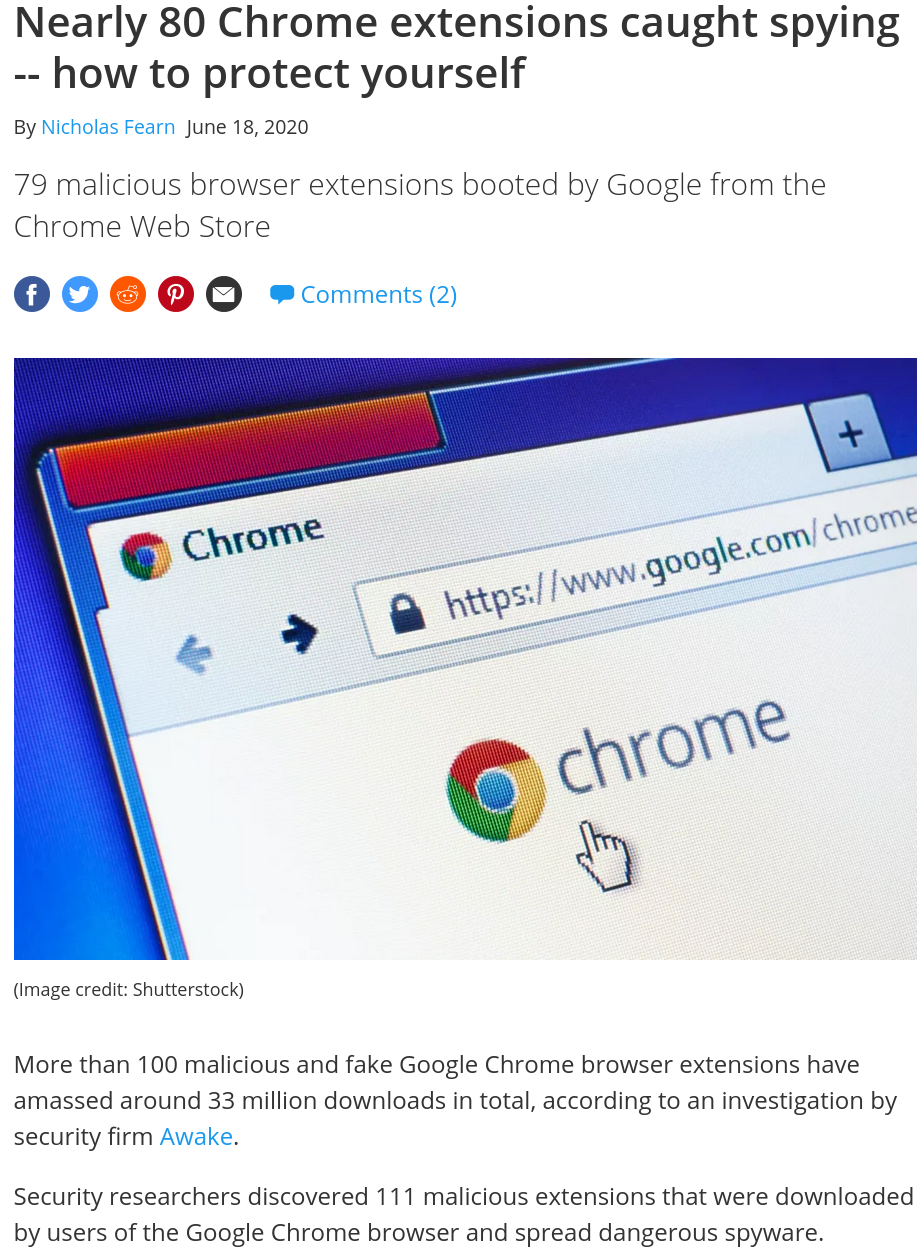
\includegraphics[height=\paperheight]{../intro/chrome-ext-article}
            };
        \end{tikzpicture}
    \end{frame}
}

